
\section{Neulesuunnittelukilpailu}\label{sec:neulekilpailu}

\begin{wrapfigure}{r}{0.25\textwidth}
	\noindent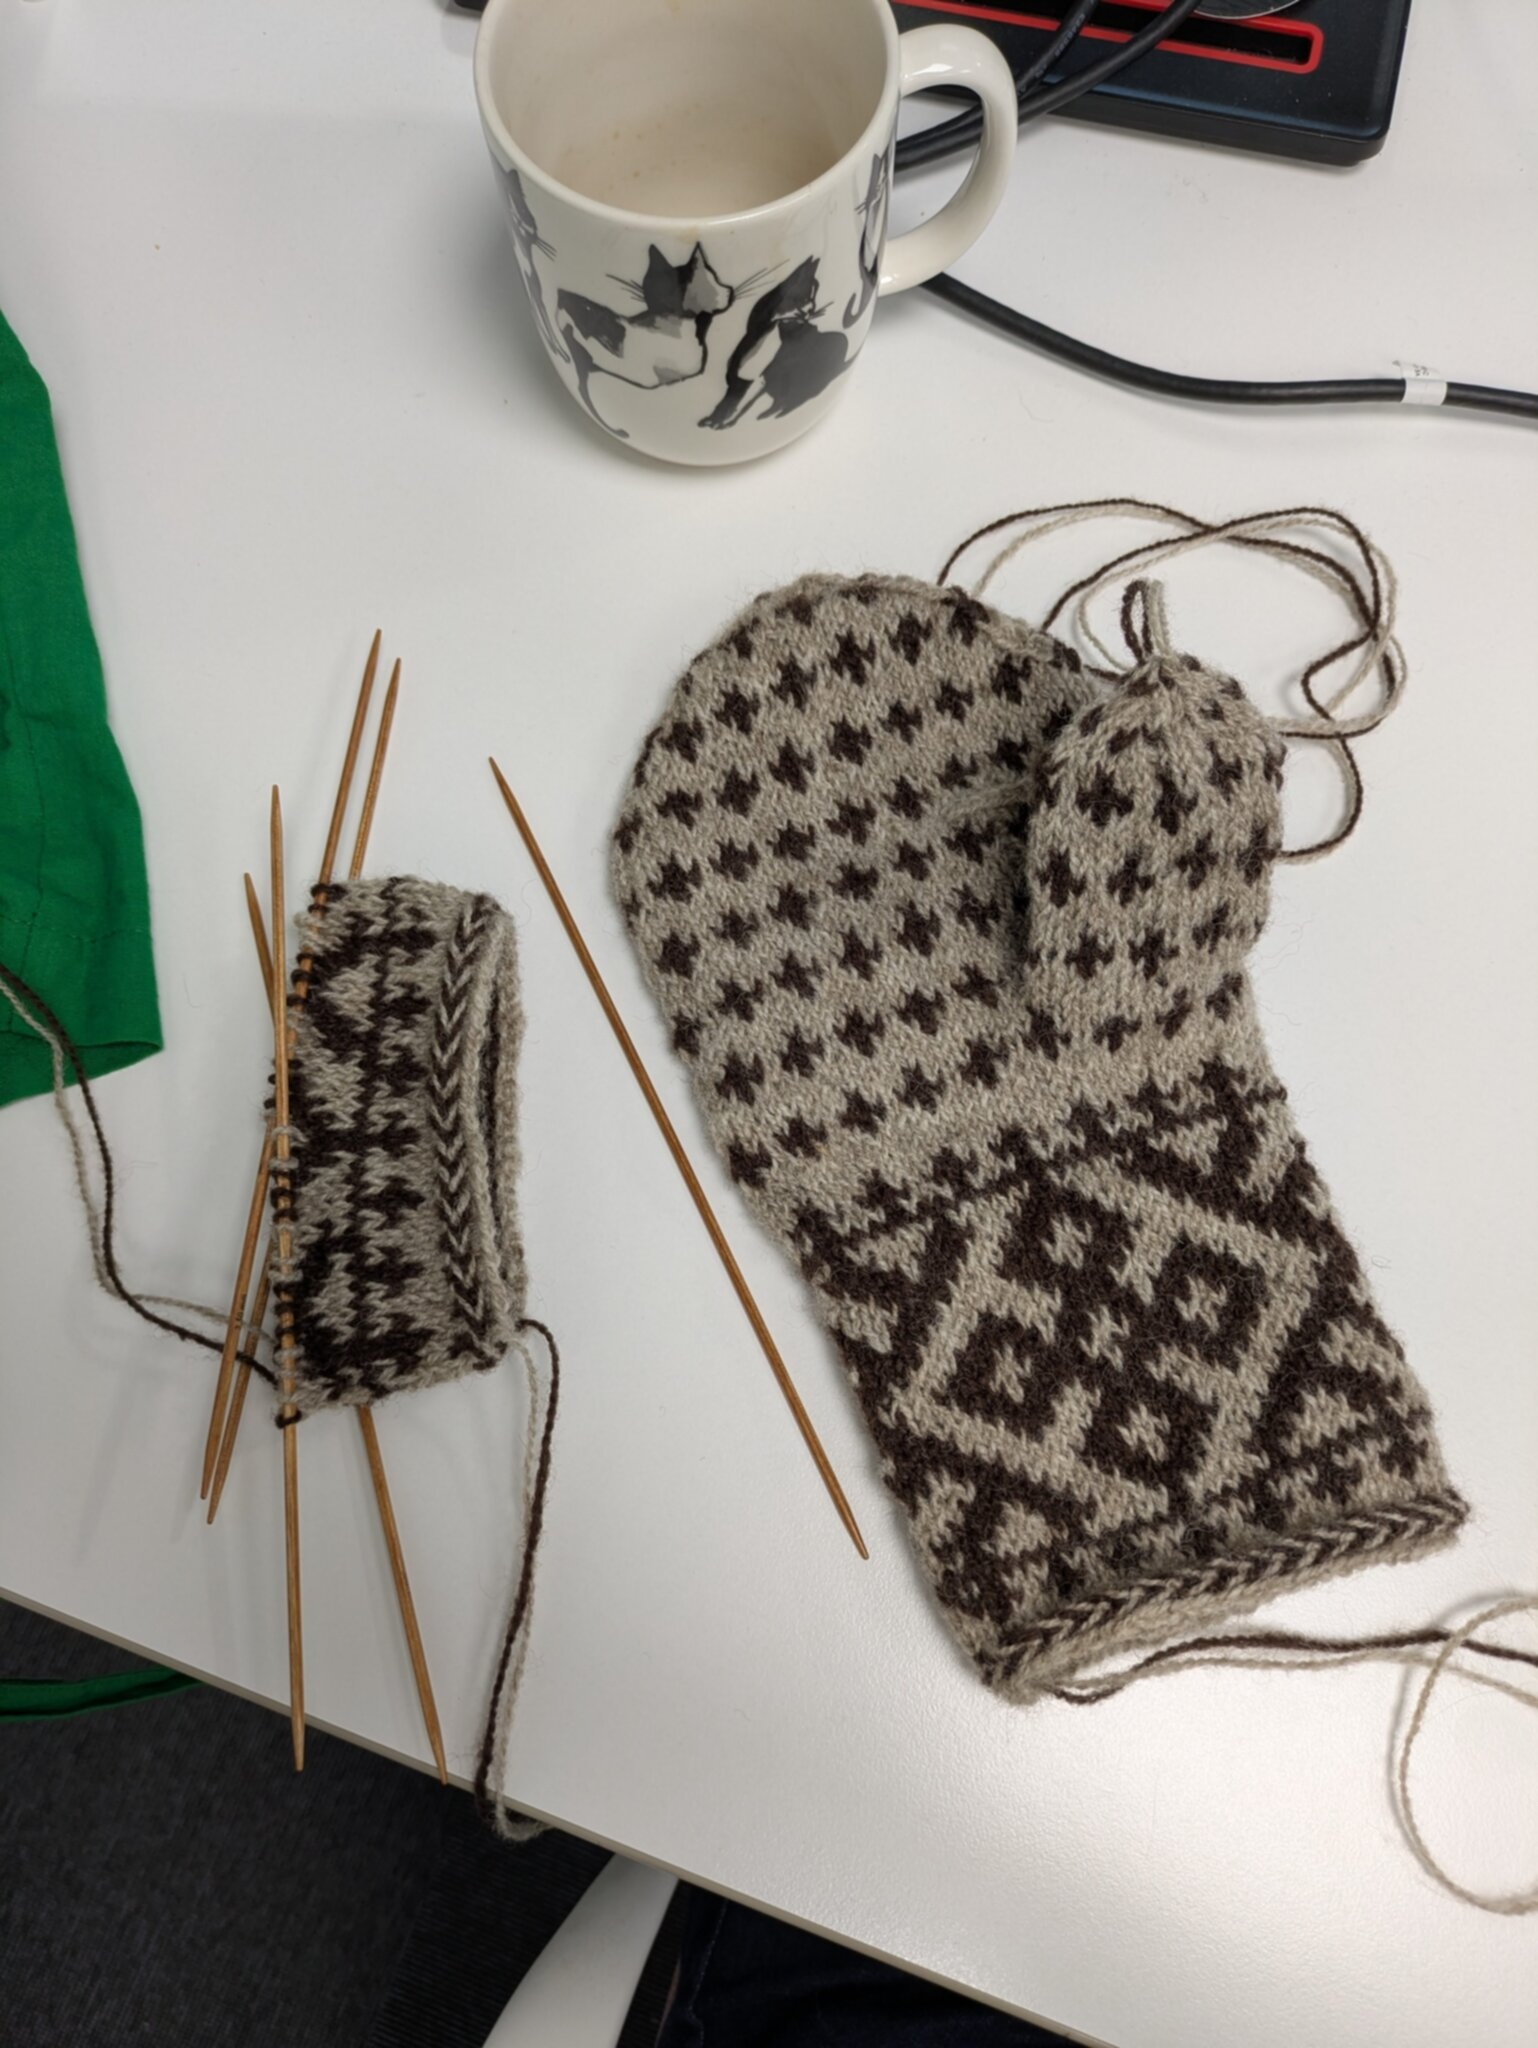
\includegraphics[width=0.9\linewidth]{assets/neulekilpailu1}
\end{wrapfigure}

Osallistumalla Tassun seuraavaan kilpailuun saatat ehkä olla \textbf{se},
joka suunnittelee KuRu:n seuraavan puolivirallisen vaatekappaleen. Me
ajattelimme, että olisi mukavaa saada KuRu:n oma neuleohje, jota kaikki
halukkaat jäsenet voisivat neuloa {\tiny(tai voisivat saada jonkun neulomaan
heille\ldots)} ja käyttää ylpeydellä.

Vaikka voi vaikuttaa siltä, että järjestämme kilpailun vain Anninalle,
\mbox{Nonnalle} ja Tanguylle, me haluamme, että se olisi mahdollisimman avoin
kaikille -- myös niille, joilla ei ole ollenkaan kokemusta neulesuunnittelusta
eikä neulomisesta. Täysin valmista neulepiirrosta ei tarvitse palauttaa eikä
\mbox{tarkkoja} silmukkalukuja ja kaikkea muuta. Jos sinulla on visio,
piirustuksia tai vain ideoita, kaikki käy, ja voidaan yhdessä valmistella
täydelliset ohjeet sen jälkeen, kun voittaja on valittu.

Vaatekappaleen tyyppi jätetään osallistujan päätettäväksi, mutta toivomme,
että se olisi sellainen, että useimmat voisivat toteuttaa sen olematta
konkareita, esimerkiksi lapaset, sukat, pipo, huivi tai vaikkapa kypärämyssy!

Arvostelemme ehdotukset kolmen kriteerin perusteella: Ehdotuksen kauneus (hyvin subjektiivista, kyllä kyllä), sen neulomisen helppous ja \mbox{''KuRu:maisuus''}.

Osallistu kilpailuun lähettämällä ehdotuksesi Tassun päätoimittajalle
sähköpostilla (osoitteen löydät lehden sisäkannesta) tai suoraan esimerkiksi
Whatsapp"-viestillä. Julkaisemme voittajan seuraavassa Tassussa.

\vfill

\begin{center}
	\noindent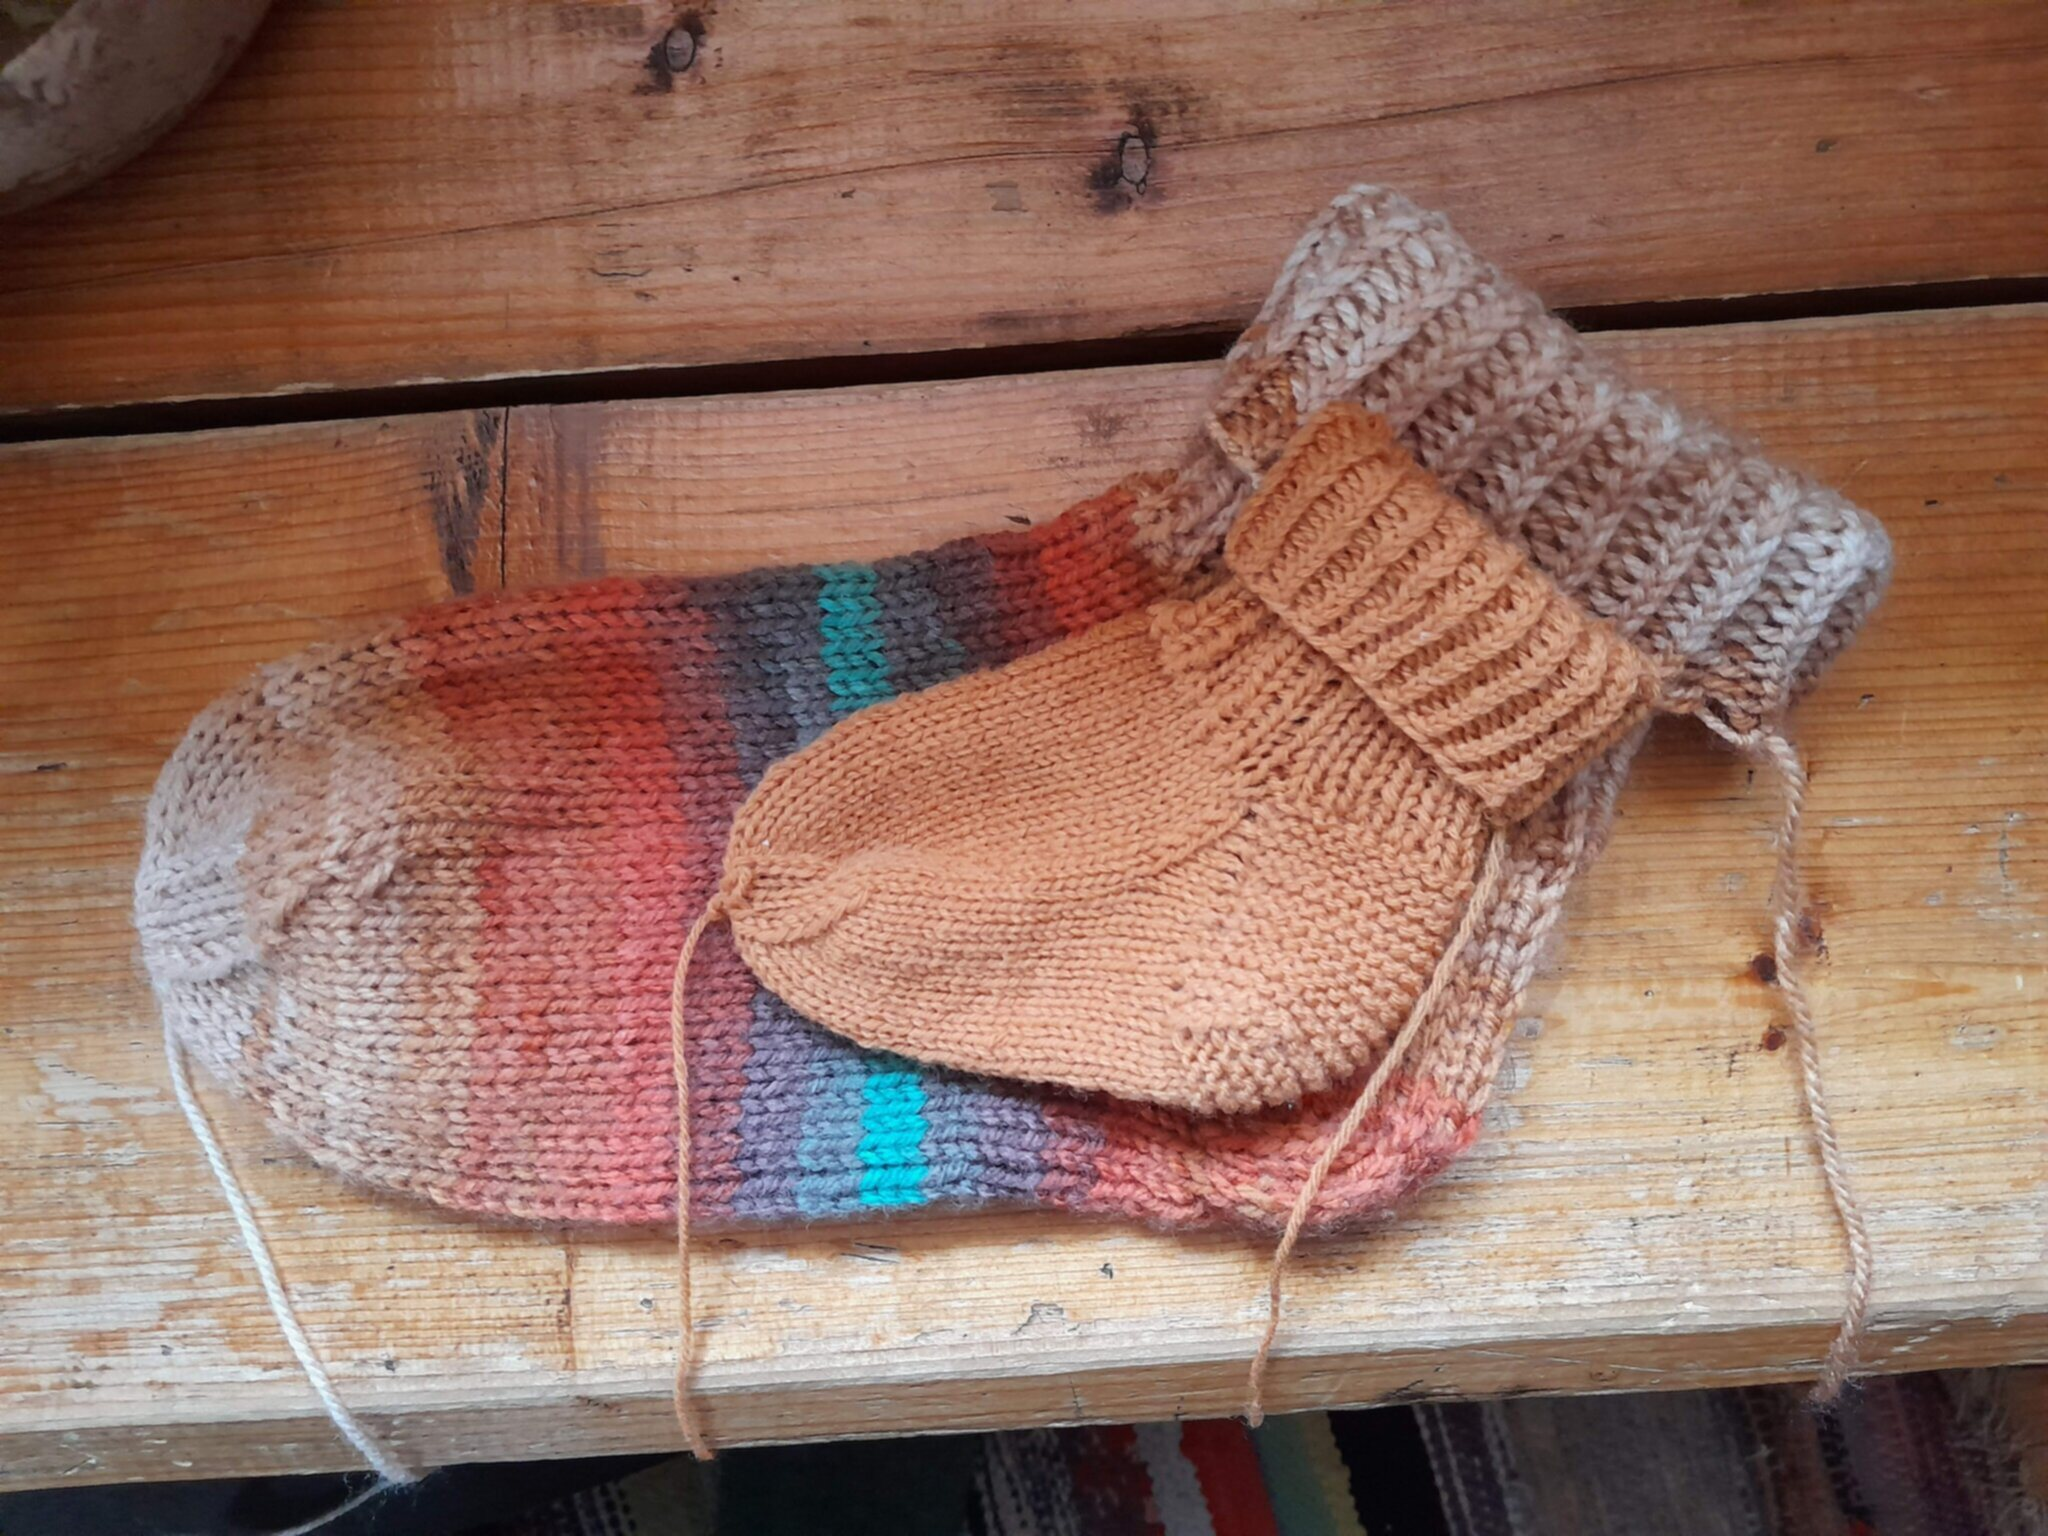
\includegraphics[width=0.8\linewidth,trim={0 9cm 0 9cm},clip]{assets/neulekilpailu2}
\end{center}
